

\begin{center}
\fbox{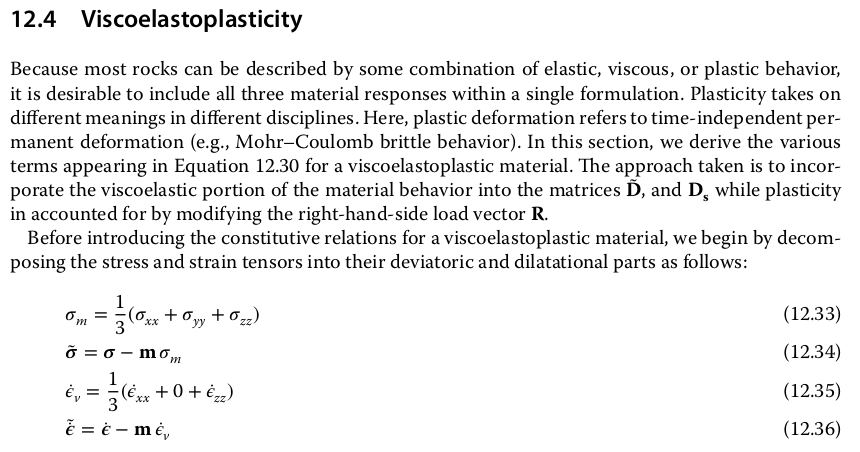
\includegraphics[width=12cm]{images/viscoelasticity/simp1}}
\end{center}

\[
\sigma_m=\frac13 {\rm tr} ({\bm \sigma})
\]



\begin{center}
\fbox{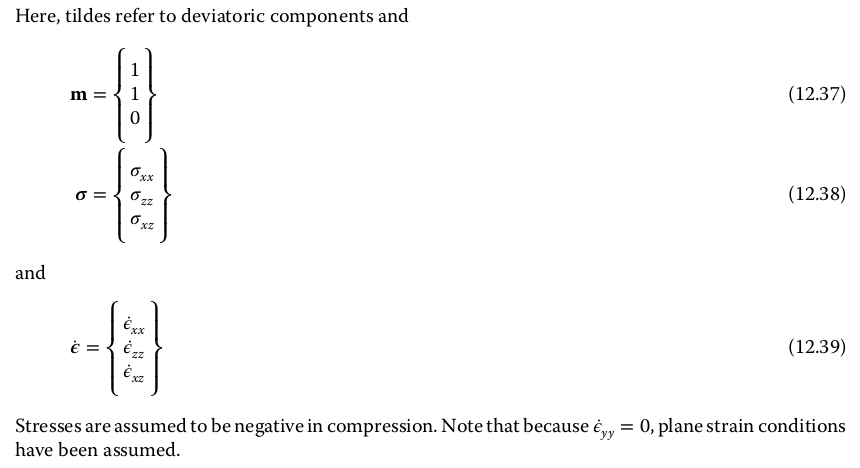
\includegraphics[width=12cm]{images/viscoelasticity/simp2}}
\end{center}

\begin{center}
\fbox{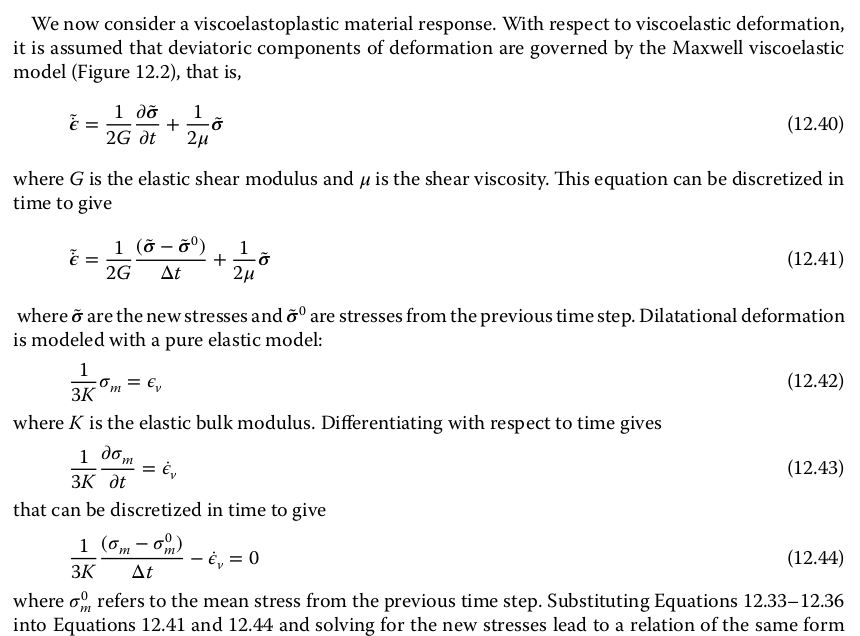
\includegraphics[width=12cm]{images/viscoelasticity/simp3}}
\end{center}

As stated above tildes refer to deviatoric components, so that 
we have 
\[
\dot{\bm\varepsilon}^d = \frac{1}{2\mu} \frac{\partial {\bm \tau}}{\partial t} + 
\frac{1}{2\eta} {\bm \tau}
\] 
We see that the use of only a partial derivative constitue a 
very crude simplication. 

Dilatational deformation is modeled with a pure elastic model:
\[
\frac{1}{K} \sigma_m= {\rm tr}({\bm \varepsilon})
\]
\[
\frac{1}{K} \frac{\partial \sigma_m}{\partial t} = {\rm tr}(\dot{\bm \varepsilon})
\]
where $K$ is the elastic bulk modulus.

where do the 3 go?!

\begin{center}
\fbox{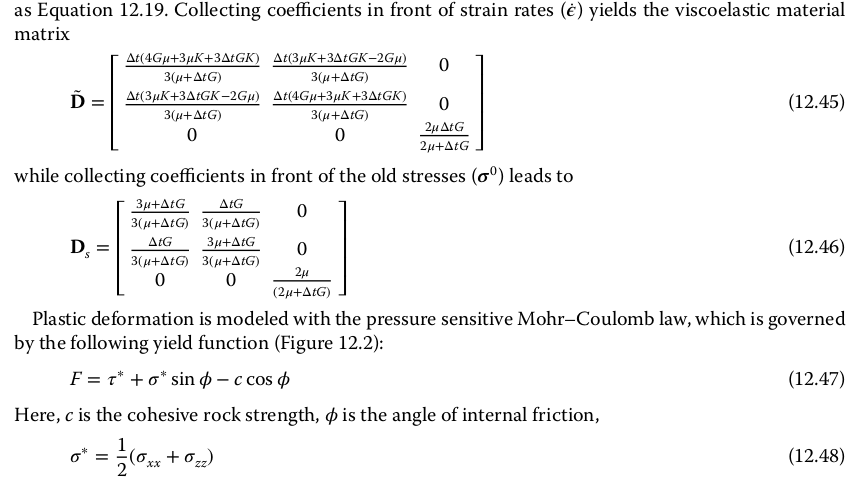
\includegraphics[width=12cm]{images/viscoelasticity/simp4}}
\end{center}

\begin{center}
\fbox{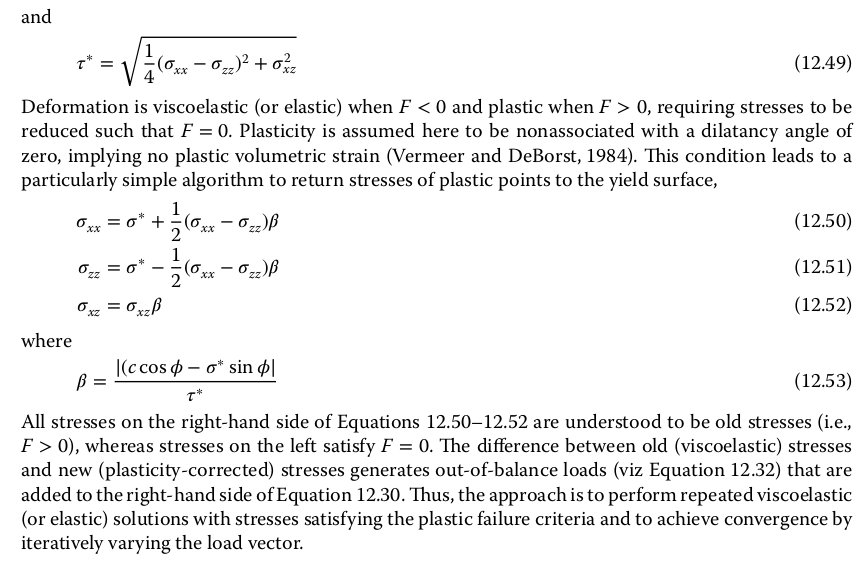
\includegraphics[width=12cm]{images/viscoelasticity/simp5}}
\end{center}


